\section{METHODOLOGY}\label{sec:methodology}
To formulate the control law of the trifocal tensor based visual servoing \eqref{eq:tensorcontrollaw}, we need to establish the model of the system and find the relation between the input of the control and the trifocal tensor coefficients. That is to find the interaction matrix relating the control input and the tensor coefficients derivatives. The error will be the difference between the current tensor and the desired tensor values.
\begin{equation}
  \begin{gathered}
  \dot{\mathcal{T}}_{(jkl)} = L_{\mathcal{T}_{(jkl)}} u_c\\
  u_c = -\lambda L_{\mathcal{T}_{(jkl)}}^{+} e
\end{gathered} \label{eq:tensorcontrollaw}
\end{equation}

\subsection{Interaction Matrix}
First, The derivatives of all the trifocal tensor elements with respect to time are generally as following:
\begin{equation}
  \begin{gathered}
  \dot{\mathcal{T}}_{(jkl)} = \tensor[^{c}]{\dot{R}}{_{c^{*}(kj)}} \tensor[^{i}]{t}{_{c^{*}(l)}} + \tensor[^{c}]{R}{_{c^{*}(kj)}} \tensor[^{i}]{\dot{t}}{_{c^{*}(l)}}\\ - \tensor[^{c}]{\dot{t}}{_{c^{*}(k)}} \tensor[^{i}]{R}{_{c^{*}(lj)}} - \tensor[^{c}]{t}{_{c^{*}(k)}} \tensor[^{i}]{\dot{R}}{_{c^{*}(lj)}} \end{gathered}\label{eq:tensorderivatives1}
\end{equation}

Since our initial camera $C_i$ is fixed, the elements of the derivatives of its rotation matrix and its transpose vector are equal to zero, \textit{i.e.:} $\tensor[^i]{\dot{t}}{_{c^{*}(l)}} = \tensor[^i]{\dot{R}}{_{c^{*}(jl)}} = 0$. Our trifocal tensor elements derivative is then simplified to:
\begin{equation}
  \dot{\mathcal{T}}_{(jkl)} = \tensor[^{c}]{\dot{R}}{_{c^{*}(kj)}} \ \tensor[^{i}]{t}{_{c^{*}(l)}} - \tensor[^{c}]{\dot{t}}{_{c^{*}(k)}} \ \tensor[^{i}]{R}{_{c^{*}(lj)}} \label{eq:tensorderivatives2}
\end{equation}

The spatial velocity of the camera is $u_c = {(v_c, \omega_{c})}^{T}$, where $v_c$ and $\omega_c$ are the translational and rotational velocities of the camera. From the geometry of the scene, we can deduce the following relationships:
\begin{gather*}
  {[\omega_{c}]}_{\times} = \tensor[^{c^*}]{R}{_{c}^{T}} \tensor[^{c^*}]{\dot{R}}{_{c}} = - \tensor[^{c^*}]{\dot{R}}{_{c}^{T}} \tensor[^{c^*}]{R}{_{c}}\\
  \tensor[^{c^*}]{\dot{R}}{_{c}^{T}} = - {[\omega_{c}]}_{\times}\tensor[^{c^*}]{R}{_{c}^{T}}\\
  \tensor[^{c^*}]{\dot{R}}{_{c}^{T}} = - {[\omega_{c}]}_{\times}\tensor[^{c}]{R}{_{c^*}}\\
  \tensor[^{c}]{\dot{R}}{_{c^*}} = -{[\omega_c]}_{\times}\tensor[^{c}]{R}{_{c^*}}
  \end{gather*}
  Similarly, we have \cite{chaumette2006visual}:
  \begin{gather*}
  \tensor[^{c^*}]{\dot{t}}{_{c}} = \tensor[^{c^*}]{R}{_{c}}v_{c}, \tensor[^{c}]{t}{_{c^*}} = - \tensor[^{c}]{R}{_{c^*}} \tensor[^{c^*}]{t}{_{c}}\\
  \tensor[^{c}]{\dot{t}}{_{c^*}} = - \tensor[^{c}]{\dot{R}}{_{c^*}} \tensor[^{c^*}]{t}{_{c}} - \tensor[^{c}]{R}{_{c^*}} \tensor[^{c^*}]{\dot{t}}{_{c}}\\
  \tensor[^{c}]{\dot{t}}{_{c^*}} = {[\omega_c]}_{\times}\tensor[^{c}]{R}{_{c^*}} \tensor[^{c^*}]{t}{_{c}} - \tensor[^{c}]{R}{_{c^*}} \tensor[^{c^*}]{R}{_{c}}v_{c}\\
  \tensor[^{c}]{\dot{t}}{_{c^*}} = {[\omega_c]}_{\times}\tensor[^{c}]{t}{_{c^*}} - v_{c}\\
  \tensor[^{c}]{\dot{t}}{_{c^*}} = {[\tensor[^{c}]{t}{_{c^*}}]}_{\times}\omega_c - v_{c}\\
  \tensor[^{c}]{\dot{t}}{_{c^{*}(k)}} = [-I | {[\tensor[^{c}]{t}{_{c^*}}]}_{\times}] u
\end{gather*}

Substituting back into the tensor derivation \eqref{eq:tensorderivatives2}, we get:
\begin{equation}
\begin{gathered}
  \dot{\mathcal{T}}_{(jkl)} =  - {({[\omega_c]}_{\times}\tensor[^{c}]{R}{_{c^*}})}_{(kj)}\ \tensor[^{i}]{t}{_{c^*(l)}} \\- {({[\tensor[^{c}]{t}{_{c^*}}]}_{\times}\omega_c - v_{c})}_{(k)}\ \tensor[^{i}]{R}{_{c^*(lj)}}\\
  \dot{\mathcal{T}}_{(jkl)} =  - (\sum_{m}{[\omega_{c}]}_{\times(km)}\tensor[^{c}]{R}{_{c^*(mj)}})\ \tensor[^{i}]{t}{_{c^*(l)}} \\- ({({[\tensor[^{c}]{t}{_{c^*}}]}_{\times}\omega_c)}_{(k)}  -   v_{c(k)})\ \tensor[^{i}]{R}{_{c^*(lj)}}
\end{gathered}\label{eq:tensorderivatives3}
\end{equation}

From~\eqref{eq:tensorcoeffs} and~\eqref{eq:tensorderivatives3}, we can compute the derivatives for all the coefficients, and deduce this compact form:
\begin{equation}
  \dot{\mathcal{T}}_{(jkl)} = R_{i(lj)}v_{c(k)} - \sum_{m} {[\omega_{c}]}_{\times(km)} \mathcal{T}_{(jml)}
\label{eq:tensorderivativesgeneral}
\end{equation}

To control the six degrees of freedom, at least six tensor coefficients are necessary. However, to avoid singularities, more than six tensor coefficients are considered. The interaction matrix $L_{T_{(jkl)}}$ taking into account all the tensor coefficients can be deduced from \eqref{eq:tensorderivativesgeneral}. It is important to notice that pose of the initial camera location is necessary for the computation of the interaction matrix as well as the normalization factor. It is also to be noticed there exists a decoupling between the translational velocities in the resulting interaction matrix. This decoupling ensures to obtain smooth camera trajectories for the motion in the 3D space.

\subsection{Tensor Normalization} \label{sub:tensor_normalization}
Since the trifocal tensor is computed up to a scale factor, we propose a normalization step to get a fixed scale. The normaliztion factors $\mathcal{T}_{kN}$ are used to obtain the normalized tensor $T_{jkl}$.  When the camera reaches the desired goal position, we can observe that the tensor coefficients are only related to the translation of the camera at the initial position which is a constant value vector. Also from~\eqref{eq:tensorderivativesgeneral}, the first column elements $\mathcal{T}_{(111)}$, $\mathcal{T}_{(112)}$, $\mathcal{T}_{(113)}$, $\mathcal{T}_{(211)}$, $\mathcal{T}_{(212)}$, $\mathcal{T}_{(213)}$, $\mathcal{T}_{(311)}$, $\mathcal{T}_{(312)}$, $\mathcal{T}_{(313)}$ are respectively equal to $\tensor[^{i}]{t}{_{c^*(1)}}$, $\tensor[^{i}]{t}{_{c^*(2)}}$, $\tensor[^{i}]{t}{_{c^*(3)}}$, $0$,$0$,$0$,$0$,$0$,$0$ at the desired goal position.

Choosing the elements $\mathcal{T}_{(111)}$, $\mathcal{T}_{(112)}$, $\mathcal{T}_{(113)}$ as normalization factors would seem a good choice for our method, as we would be interested in coefficients converging to non-zero values. However, it was found that for some scene configurations, these three coefficients could have values equal to zero at the initial pose. Which means at normalization step, this would cause dividing by a zero value. To avoid this problem, we will use all the nine coefficients of the first column to be our first normalization factor. We can then normalize the elements $T_{jkl}$ for $k = 1$ as follows:
\begin{equation}
  \begin{gathered}
    T_{jkl} = \frac{\mathcal{T}_{jkl}}{\mathcal{T}_{1N}}\\
    \mathcal{T}_{1N} = ({\mathcal{T}_{111}}^{2}+{\mathcal{T}_{112}}^{2}+{\mathcal{T}_{113}}^{2}+{\mathcal{T}_{211}}^{2}+{\mathcal{T}_{212}}^{2}+{\mathcal{T}_{213}}^{2} \\+ {\mathcal{T}_{311}}^{2}+{\mathcal{T}_{312}}^{2}+{\mathcal{T}_{313}}^{2}) ^{\frac{1}{2}}
  \end{gathered}
\end{equation}

Unfortunately, this normalization factor is dependent on the tensor coefficients which varies with time. So we need to find also the derivative of the normalization factor.
A general formula for $\dot{T}_{(jkl)}$ can then be found as following
\begin{equation}
  \begin{gathered}
    \dot{T}_{(jkl)} = \frac{\tensor[^{i}]{R}{_{c^{*}(lj)}}}{\mathcal{T}_{kN}}v_{c(k)} -T_{(jkl)}(\sum_n \sum_{m}T_{nkm}\frac{\tensor[^{i}]{R}{_{c^{*}(mn)}}}{\mathcal{T}_{kN}}) v_{c(k)}\\ + T_{(jkl)}(\sum_n \sum_{m}T_{nkm}T_{nhm})\omega_{(g)} \\- T_{(jkl)}(\sum_n \sum_{m}T_{nkm}T_{ngm})\omega_{(h)} \\+\sum_{m} {[\omega_{c}]}_{\times(km)} T_{(jml)}\\
      \text{where } g = k\%3 +1, h = (k+1)\%3 +1
  \end{gathered}\label{eq:tensornormalizationgeneral}
\end{equation}

From \eqref{eq:tensornormalizationgeneral}, the final normalized interaction matrix can be computed. As we notice, this particular choice for the normalization factors has led to keep the decoupling property between the translational velocities, as each degree of freedom related tensor coefficients are normalized separately from other degrees of freedom. Other choices of different combinations of tensor coefficients as normalization factors, would introduce extra non-zero elements to the normalized interaction matrix and prevent keeping the decoupling property.

\subsection{Proposed Method}
We have defined all the elements of the control law \eqref{eq:tensorcontrollaw}. The interaction matrix $L_{T_{(jkl)}}$ is computed as indicated in \eqref{eq:tensornormalizationgeneral}. The error $e$ is computed using the difference between the current tensor coefficients and the desired tensor coefficients, $e = T_{(jkl)} - T_{(jkl)}^{*}$. In Figure \ref{fig:vsttloop}, we present the block diagram explaining the proposed trifocal tensor visual servoing control loop. At initialization, the desired tensor $T_{(jkl)}^{*}$ is computed from feature correspondences across three images obtained from the three camera poses: initial pose, desired pose, and current pose being equal to the desired pose.
\begin{figure*}[ht!]
  \centering
  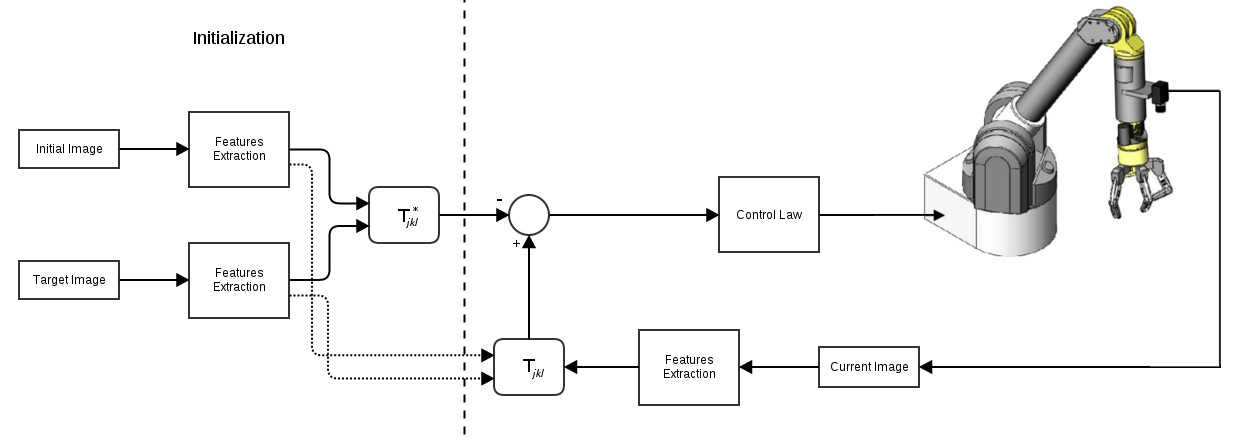
\includegraphics[width=150mm,height=50mm]{figures/vsttloop.png}
  \caption{Block diagram of the proposed Trifocal Tensor Visual Servoing loop control}
  \label{fig:vsttloop}
\end{figure*}

The current tensor $T_{(jkl)}$ is computed inside the visual servoing loop at each iteration. Then the interaction matrix is computed using the current tensor. For simplicity, we make the assumption that the initial pose is known and the interaction matrix can be computed directly. The new error value is computed along with the pseudo-inverse of the interaction matrix and fed back to the control law to compute the required velocities to drive the camera to the desired pose. The system converges and the loop is terminated when the camera reaches the desired pose. This is evaluated when the sum squared of the error reaches a value less than a defined threshold, $1 \times \e{-6}$ for example.
